\documentclass[a4paper]{article}
\usepackage[utf8]{inputenc}
\usepackage[italian]{babel}
\usepackage{import}
\usepackage{graphicx}
\usepackage{float}
\usepackage[margin=1.2in]{geometry}
\usepackage[12pt]{extsizes}
\usepackage{color}
\usepackage{listings}
\usepackage[bottom,flushmargin,hang,multiple]{footmisc}
\usepackage{titlesec}
\usepackage{url}
\usepackage{upquote}
\usepackage{csquotes}
\usepackage{biblatex}
\usepackage{spverbatim}
\usepackage{dirtree}
\usepackage{dirtree}
\usepackage{etoolbox}
\apptocmd{\dirtree}{\bigskip}{}{}
\pretocmd{\dirtree}{\bigskip}{}{}
\definecolor{purple}{RGB}{91, 72, 181}
\definecolor{darkviolet}{rgb}{0.58, 0.0, 0.83}
\definecolor{royalblue}{RGB}{242, 73, 214}
\definecolor{orange}{RGB}{227, 72, 41}
\definecolor{lightgreen}{RGB}{164, 194, 14}

\definecolor{mediumgray}{rgb}{0.3, 0.4, 0.4}
\definecolor{forestgreen}{rgb}{0.13, 0.55, 0.13}
\definecolor{crimson}{rgb}{0.86, 0.8, 0.24}

\addbibresource{./bibliografia/bibliografia.bib}

\linespread{1.5}
\graphicspath{ {./images/} }

\setcounter{secnumdepth}{4}
\setcounter{tocdepth}{4}

\titleformat{\paragraph}{\normalfont\normalsize\bfseries}{\theparagraph}{1em}{}
\titlespacing*{\paragraph}{0pt}{3.25ex plus 1ex minus .2ex}{1.5ex plus .2ex}

\lstset{aboveskip=30pt,belowskip=30pt}

\lstdefinestyle{JSES6Base}{
  backgroundcolor=\color{white},
  basicstyle=\ttfamily,
  breakatwhitespace=false,
  breaklines=true,
  captionpos=b,
  columns=fullflexible,
  commentstyle=\color{mediumgray}\upshape,
  emph={},
  emphstyle=\color{crimson},
  extendedchars=true,  % requires inputenc
  fontadjust=true,
  frame=single,
  identifierstyle=\color{black},
  keepspaces=true,
  keywordstyle=\color{purple},
  keywordstyle={[2]\color{darkviolet}},
  keywordstyle={[3]\color{royalblue}},
  keywordstyle={[4]\color{orange}},
  keywordstyle={[5]\color{lightgreen}},
  numbers=left,
  numbersep=5pt,
  numberstyle=\tiny\color{black},
  rulecolor=\color{black},
  showlines=true,
  showspaces=false,
  showstringspaces=false,
  showtabs=false,
  stringstyle=\color{forestgreen},
  tabsize=2,
  title=\lstname,
  upquote=true  % requires textcomp
}

\lstdefinestyle{JavaScript}{
  language=JavaScript,
  style=JSES6Base
}

\lstdefinestyle{ES6}{
  language=ES6,
  style=JSES6Base
}

\lstdefinelanguage{JavaScript}{
  morekeywords=[1]{break, continue, delete, else, for, function, if, in,
    new, return, this, typeof, var, void, while, with, render, getElementById, width, height, contract, address, event, uint256, public, returns, emit, pragma, describe, it},
  % Literals, primitive types, and reference types.
  morekeywords=[2]{false, null, true, boolean, number, undefined,
    Array, Boolean, Date, Math, Number, String, Object, onClick, Map, onChange, SMART_CONTRACTS, TKN_TMPLT_ABI, SALE_FCTRY_ADDR, SALE_FCTRY_ABI},
  morekeywords=[3]{h1, div, p, button, TextField},
  morekeywords=[4]{React, ., Component, Saluto, Convenevoli, Contatore, setContatore, useState, contatore,
    Button, ContatoreConTitolo, handleSearch, searchInput, target, value, setActiveCoinsList, coinsList, coinName, coinSymbol, coin,
    coinsToSellAmounts, setCoinsToSellAmounts, coinsToAcceptAmounts, setCoinsToAcceptAmounts, setCoinsList, activeCoinsList,
    activeStep, setActiveStep, web3Instance, userAccount, fetchCoins, setLoadingCoinList, newCoinsList, Contratto, saleCreate, web3,
    sellerAddress, coinsOnSaleAddr, amountsOnSale, coinsToAcceptAddr, amountsToAccept, expirationDate, coinInstance, SaleFactoryInstance, creationResponse, saleAddr},
  morekeywords=[5]{},
  sensitive,
  morecomment=[s]{/*}{*/},
  morecomment=[l]//,
  morecomment=[s]{/**}{*/}, % JavaDoc style comments
  morestring=[b]',
  morestring=[b]"
}[keywords, comments, strings]

\lstalias[]{ES6}[ECMAScript2015]{JavaScript}

\lstdefinelanguage[ECMAScript2015]{JavaScript}[]{JavaScript}{
  morekeywords=[1]{await, async, case, catch, class, const, default, do,
    enum, export, extends, finally, from, implements, import, instanceof,
    let, static, super, switch, throw, try},
  morestring=[b]` % Interpolation strings.
}


\title{Progettazione e realizzazione di un exchange decentralizzato per lo scambio di token ERC20 per la piattaforma CommonsHood}

\begin{document}
    \tableofcontents
    \newpage
    \section{Background}
    \subsection{CommonsHood}
    CommonsHood è un’applicazione web basata su smart contract per blockchain Ethereum che ha lo scopo di fornire alla comunità strumenti per l’inclusione finanziaria e per supportare l’economia locale delle comunità di cittadini.
    Gli utenti, una volta registrati sulla piattaforma, possono creare monete, ossia token crittografici Ethereum basati sullo standard ERC-20, questi possono rappresentare beni di valore o servizi.
    Un altro asset che gli utenti possono creare e possedere sono i coupon, questi sono rappresentati da token non fungibili basati sullo standard ERC-721, in questo modo ogni singolo coupon è univoco e diverso dagli altri.
    Gli utenti possono utilizzare i coupon per ottenere prestazioni e servizi.
    \newline
    Un'altra funzionalità offerta dall'applicazione è la possibilità di creare crowdsales, questi sono usati per ottenere fondi per finanziare progetti o eventi, dando, in cambio, ai finanziatori monete oppure coupons.
    Un esempio di un'interazione con la piattaforma potrebbe essere: il negozio di attrezzature da sub \emph{"Sotto il Mar"} crea un account su CommonsHood. Crea, inoltre, una moneta chiamata \emph{"Doblone"}, questa può essere spesa in negozio
    per acquistare le attrezzature. Oltre alla vendita, il negozio noleggia anche le attrezzature, perciò crea dei coupon che possono essere utilizzati per ottenere i prodotti a noleggio.
    Inoltre, una stanza ha bisogno di ristrutturazioni perciò viene creata una crowdsale per ottenere il finanziamento necessario, in cambio vengono offerti dei coupon del negozio.
    
    \subsection{Blockchain}
    Una blockchain è un registro aperto e distribuito di dati, strutturato come una catena di blocchi contenenti le transazioni.
    Le transazioni solitamente rappresentano uno scambio di monete, chiamate token. Ogni blockchain ha un token proprio.
    I dati risiedono su unità computazionali chiamati \emph{nodi}, questi, come mostrato nell'immagine \ref{fig:node},
    sono interconnessi e comunicano tra loro per mantenere i dati di tutti i nodi aggiornati\cite{nodo}.
    Un account su una blockchain è costituito da una coppia di chiavi:
    \begin{itemize}
      \item pubblico: è un indirizzo sulla blockchain, i token nella rete sono registrati come appartenenti ad un indirizzo;
      \item privato: è come una password che l'utente utilizza per accedere ai propri fondi.
    \end{itemize}
    \begin{figure}[ht]
      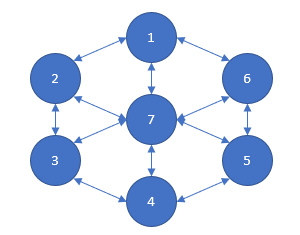
\includegraphics[scale=0.8]{node.png}
      \centering
      \caption{Rete di nodi}
      \centering
      \label{fig:node}
    \end{figure}
    \subsubsection{I nodi}
    Le responsabilità di un nodo sono principalmente:
    \begin{itemize}
      \item Controllo della validità di un nuovo record di dati, chiamato anche transazione, e accettarlo o rifiutarlo;
      \item Nel caso di un record valido, salvataggio della transazione nel registro locale del nodo;
      \item Comunicazione e distribuzione della transazione agli altri nodi. In questo modo tutti i nodi hanno la stessa versione del registro.
    \end{itemize}
    \subsubsection{Le caratteristiche di una blockchain}
    Le caratteristiche principali della tecnologia blockchain sono:
    \begin{itemize}
      \item Decentralizzazione: le informazioni contenute nel registro digitale vengono distribuite tra più nodi, così da garantire sicurezza e resilienza dei sistemi anche in caso di attacco a uno dei nodi o in caso di perdita di un nodo.
      \item Tracciabilità: ogni elemento salvato nel registro è tracciabile in ogni sua parte e se ne può risalire all’esatta provenienza e alle eventuali modifiche apportate nel corso del tempo, con una precisione assoluta.
      \item Disintermediazione: i singoli nodi della blockchain certificano le informazioni distribuite, rendendo quindi del tutto inutile la presenza di enti centrali o di aziende per la certificazione dei dati.
      \item Trasparenza: il contenuto del registro è visibile a tutti ed è facilmente consultabile e verificabile da ogni nodo della rete ma anche tramite servizi che interrogano la blockchain senza apportare modifiche. Nessuno può nascondere o modificare dati senza che l'intera rete venga a saperlo.
      \item Solidità del registro: dopo aver aggiunto un'informazione al registro, essa non può essere modificata senza il consenso di tutta la rete.
      \item Programmabilità: le operazioni di transazione possono anche essere programmate nel tempo, così da poter attendere il verificarsi di determinate condizioni prima di procedere con l'inserimento o la modifica\cite{blockchain1}.
    \end{itemize}
    \subsubsection{Smart contracts}
    Le blockchain permettono d'implementare codici e funzioni all'interno di esse, questi sono chiamati smart contracts e permettono l'esecuzione di operazioni quando predeterminate condizioni si avverano.
    Sono tipicamente usate per automatizzare l'esecuzione di un accordo, in questo modo tutti i partecipanti possono verificarne immediatamente i risultati, senza aver bisogno di un intermediario.
    Possono, inoltre, essere utilizzate per automatizzare workflow, innescando azioni successive al raggiungimento di certe condizioni\cite{smartcontracts}.
    
    \subsection{Ethereum}
    Ethereum è una piattaforma blockchain decentralizzata che stabilisce una rete peer-to-peer che esegue e verifica smart contracts in modo sicuro.
    Gli smart contracts permettono transazioni tra gli utenti senza la necessità di un autorità centrale.
    Le transazioni sono immutabili, verificabili, e distribuiti in modo sicuro sulla rete. Le transazioni sono inviate e ricevute da account Ethereum creati dagli utenti.
    Come costo per il processamento di una transazione sulla rete, l'utente deve spendere Ether (ETH), la criptovaluta nativa di Ethereum\cite{ethereum}.
    \subsubsection{Token Ethereum}
    Ethereum permette la creazione di token crittografici all'interno della sua rete. Questi token non sono altro che smart contracts scritti seguendo specificazioni stabilite
    dagli sviluppatori della rete. I token possono essere di tipi di differenti, a seconda delle specificazioni seguite. In Ethereum ci sono principalmente due tipi di token: token ERC-20 e NFT.
    \paragraph{Token ERC-20}
    I token ERC-20 sono il tipo di token più diffuso sulla rete Ethereum, sono lo standard per la definizione di token fungibili\cite{erc20}, ossia i singoli token sono indistinguibili e intercambiabili tra loro.
    Un token ERC-20 implementa le specificazioni indicate nell'EIP-20\footnote{Ethereum Improvement Proposal} che richiede nello smart contract del token la presenza di diversi metodi. I più importanti metodi richiesti sono:
    \begin{itemize}
      \item \verb|balanceOf(address _owner)|: restituisce la quantità di token posseduto da \verb|_owner|;
      \item \verb|transfer(address _to, uint256 _value)|: trasferisce una quantità di token indicata da \verb|_value| all'indirizzo \verb|_to|;
      \item \verb|transferFrom(address _from, address _to, uint256 _value)|:\newline trasferisce una quantità \verb|_value| di token dall'indirizzo \verb|_from| all'indirizzo \verb|_to|;
      \item \verb|approve(address _spender, uint256 _value)|: permette all'indirizzo \verb|_spender| di ritirare fino a \verb|_value| token dall'account\cite{eip20}.
    \end{itemize}

    \paragraph{NFT}
    I Non Fungible Tokens sono, appunto, token non fungibili, ossia ogni token è univoco e non intercambiabile con un altro. Sono utilizzati per replicare le proprietà tipiche
    di un oggetto fisico come la scarsità, l'unicità e la possibilità di dimostrare la proprietà del token\cite{nft}.
    Data la natura del token, l'uso più comune di questi token è la creazione di arte digitale\cite{nftuse}.
    \newline
    Gli NFT seguono lo standard dettato dall'EIP-721. I metodi più significativi richiesti dall'EIP-721 sono:
    \begin{itemize}
      \item \verb|balanceOf(address _owner)|: restituise il numero di NFT posseduti da \verb|_owner|;
      \item \verb|ownerOf(uint256 _tokenId)|: restituisce il proprietario del NFT identificato da \verb|_tokenId|;
      \item \verb|safeTransferFrom(address _from,address _to,uint256 _tokenId)|: trasferisce la proprietà del NFT \verb|_tokenId| da \verb|_from| a \verb|_to|.
            Fallisce se il chiamante della funzione non è il proprietario corrente, un operatore autorizzato o un indirizzato autorizzato per questo NFT.
            Inoltre, il metodo fallisce se: \verb|_from| non è il proprietario corrente, \verb|_to| è l'indirizzo zero e \verb|_tokenId| non è un NFT valido\cite{eip1155}.
    \end{itemize}
    \subsubsection{Smart contracts in Ethereum}
    In Ethereum gli smart contracts sono considerati come account, questo significa che hanno un saldo e possono inviare transazioni sulla rete. A differenza di un normale account, però,
    gli smart contracts non sono controllati dagli utenti ma eseguono il codice con cui sono stati programmati. Gli account user possono interagire con uno smart contract inviando una transazione
    che effettua una chiamata a una funzione definita nello smart contract. Di default questi contratti non possono essere eliminati e le interazioni con essi sono irreversibili.
    \newline
    Il codice di uno smart contract si scrive utilizzando \emph{Solidity}, un linguaggio object-oriented usato per implementare smart contracts su diverse piattaforme blockchain.
    Di seguito un esempio di uno smart contract semplice:
    \begin{lstlisting}[style=ES6, title={Esempio codice di uno smart contract}]
      pragma solidity ^0.5.2;

      contract EsempioContratto() {
        address public owner;
        
        event EsempioEvento(
          uint256 parametroEvento
        )

        function esempioFunzione(
          uint256 _parametro
        ) public returns (uint256) {
          emit EsempioEvento(_parametro)
          return _parametro
        }
      }\end{lstlisting}
      Solitamente uno smart contract inizia con la dichiarazione della versione di solidity usata per la scrittura del codice, in questo modo il compilatore, se di versione superiore, rifiuta la compilazione del codice.
      Per far questo si scrive: \newline \verb|pragma solidity [versione]|. Nell'esempio precedente la versione è dichiarata nella prima riga, in questo caso la versione indicata è superiore a 0.5.2.
      \newline
      Una volta dichiarata la versione, inizia il codice dello smart contract, questo viene indicato con \verb|contract [nome contratto]()|. Prendendo sempre come riferimento l'esempio precedente,
      alla riga 4 viene dichiarata una variabile chiamata owner con visibilità \verb|public| e tipo \verb|address|, ossia un indirizzo Ethereum. Ci sono 4 livelli di visibilità per le variabili e le funzioni:
      \begin{itemize}
        \item \verb|public|: le funzioni possono essere chiamate anche da contratti esterni, per le variabili vengono generate in automatico delle funzioni getter implicite;
        \item \verb|external|: le funzioni e le variabili possono essere accedute solo dall'esterno e non internamente nel contratto;
        \item \verb|internal|: le funzioni e le variabili possono essere accedute dentro il contratto stesso e i contratti derivati;
        \item \verb|private|: visibili solo nel contratto in cui le variabili e le funzioni sono definite\cite{solidityvisibility}.
      \end{itemize}
      Solidity fornisce numerosi tipi per le variabili, di cui quelle usate in questa tesi sono:
      \begin{itemize}
        \item \verb|bool|: per indicare una variabile booleana;
        \item \verb|uint|: per indicare un intero senza segno, può avere diverse dimensioni aggiungendo il numero di bits, ad esempio \verb|uint256|;
        \item \verb|address|: per indicare un indirizzo Ethereum;
        \item \verb|mapping|: per indicare un dizionario con chiavi di ricerca e valori associati\cite{soliditytypes}.
      \end{itemize}
      Alla riga 6 è stato dichiarato un evento, ossia uno strumento utile per fare logging delle transazioni e per permettere agli utenti di mettersi in ascolto di questi eventi.
      Un evento può contenere dati aggiuntivi, in questo caso l'evento \verb|EsempioEvento| contiene il dato \verb|parametroEvento| di tipo uin256.
      Per emettere un evento si utilizza \verb|emit [nome evento](dati evento)|, come mostrato alla riga 13.
      \newline
      Alla riga 10 è stata dichiarata una funzione di nome \verb|esempioFunzione|, con visibilità \verb|public|, con parametro \verb|_parametro| e che restituisce un valore di tipo \verb|uin256|.
      Questa funzione esegue solo due operazioni: emette l'evento \verb|EsempioEvento| e restituisce un valore. 

    \subsection{OpenZeppelin}
    OpenZeppelin è una libreria per lo sviluppo di smart contracts sicuri. Le principali funzionalità fornite da OpenZeppelin sono:
    \begin{itemize}
    \item Implementazione dei diversi standard dei token Ethereum;
    \item Gestione del controllo degli accessi agli smart contracts;
    \item Componenti Solidity riutilizzabili per creare smart contracts\cite{openzeppelin}.
    \end{itemize}

    \subsection{Metamask}
    Metamask è un'estensione del web browser. Questo software permette di connettere il browser con
    applicazioni decentralizzate basate sulla piattaforma Ethereum. Metamask permette la gestione di
    wallet Ethereum, la ricezione e l'invio di criptomonete basate su Ethereum, e l'interazione con
    applicazioni decentralizzate. L'estensione, inoltre, fornisce le API Ethereum web3, in questo
    modo le applicazioni sono in grado di leggere dati sulla blockchain\cite{metamask}.

    \subsection{ReactJS}
    React è una libreria JavaScript open-source per lo sviluppo d'interfacce utente.
    \subsubsection{Caratteristiche di ReactJS}
    React fornisce numerosi strumenti che facilitano lo sviluppo di un'interfaccia grafica. Di seguito sono descritti quelli utilizzati in questa tesi.
    \paragraph{Componenti}
    I Componenti permettono di suddividere la UI in parti indipendenti, riutilizzabili e di pensare a ognuna di esse in modo isolato.
    Per definire un componente è necessario implementare una funzione JavaScript, ad esempio:

    \begin{lstlisting}[style=ES6, title={Esempio componente}]
        function Saluto(props) {
            return <h1>Ciao, {props.nome}</h1>;
        }\end{lstlisting}

    Questo componente accetta un oggetto parametro contenente dati sotto forma di una singola
    "props", il quale è un oggetto parametro avente dati al suo interno.
    Per renderizzare un componente bisogna utilizzare la funzione \verb|ReactDOM.render()|,
    passandole come parametri il componente da visualizzare e il riferimento al componente padre.
    Se si volesse, quindi, renderizzare il componente \verb|Saluto|, passando "\emph{Martina}" come parametro \verb|nome|, il codice potrebbe essere:
    
    \begin{lstlisting}[style=ES6, title={Esempio composizione di componenti}]
      ReactDOM.render(
        <Saluto nome="Martina"/>, 
        document.getElementById('root')
      );\end{lstlisting}
    
    I componenti, inoltre, possono essere composte da altri componenti. In questo caso,
    renderizzando il componente padre, verranno visualizzati anche i componenti figli. Ad esempio, 
    si potrebbe avere un componente \verb|Convenevoli| che contiene multipli componenti \verb|Saluto|:
    \begin{lstlisting}[style=ES6, title={Esempio renderizzazione componente}]
      function Convenevoli() {
        return (
          <div>
            <Saluto nome="Sara" />
            <Saluto nome="Cahal" />
            <Saluto nome="Edite" />
          </div>
        );
      }\end{lstlisting}

      \paragraph{Hook state}
      Un componente React di default è stateless. Usando la funzione \verb|useState()| si può
      aggiungere uno stato interno a un componente, React preserverà questo stato tra le ri-renderizzazioni.
      \verb|useState| ritorna una coppia: il valore dello stato corrente e una funzione che ci permette di aggiornarlo.
      La funzione ha un unico parametro ed è il suo stato iniziale. Ad esempio, se si volesse realizzare un contatore con un bottone che, alla sua pressione,
      aumenti il valore del contatore, si potrebbe scrivere il seguente codice:
      \begin{lstlisting}[style=ES6, title={Esempio contatore con stato interno}]
        function Contatore() {
          const [contatore, setContatore] = useState(0);
          return (
            <div>
              <p>Hai cliccato {contatore} volte</p>
              <button 
                onClick={() => setContatore(contatore + 1)}>
                Cliccami
              </button>
            </div>
          );
        }\end{lstlisting}

      \paragraph{Hook effect}
      Il costrutto \verb|useEffect()| permette l'esecuzione di funzioni a ogni renderizzazione da parte di React.
      Questa funzione viene utilizzata per effettuare operazioni nei vari stati del ciclo di vita di un componente.
      \newline
      Nel seguente esempio il titolo del documento viene aggiornato all'aumentare del valore del contatore, infatti, 
      a ogni aggiornamento del DOM da parte di React, viene chiamata la funzione passata a \verb|useEffect()|.
      \begin{lstlisting}[style=ES6, title={Esempio uso di useEffect()}]
        function ContatoreConTitolo() {
          const [contatore, setContatore] = useState(0);

          useEffect(() => {
            document.title = `Hai cliccato ${contatore} volte`;
          });

          return (
            <div>
              <p>Hai cliccato {contatore} volte</p>
              <button
                onClick={() => setContatore(contatore + 1)}>
                Cliccami
              </button>
            </div>
          );
        }\end{lstlisting}

        \subsection{Material-UI}
        Material-UI è una libreria per ReactJS per creare interfacce utente.
        La libreria contiene al suo interno numerosi componenti grafici,
        questi sono forniti di un tema di default, per modificare l'aspetto di
        un componente si può utilizzare la sua proprietà \verb|className|.
        \newline
        Nell'esempio seguente, preso da \cite{materialui}, vengono modificati le dimensione di un componente \verb|<Button>|:
        \begin{lstlisting}[style=ES6, title={Esempio modifica aspetto di un componente}]
          .Button {
            width: "100px",
            height: "100px"
          }

          <Button className="Button">\end{lstlisting}

        \subsection{Truffle e Ganache}
        Truffle e Ganache sono entrambi strumenti contenuti all'interno della suite software Truffle.
        Ganache permette la creazione di una blockchain Ethereum che viene eseguita in locale, semplificando, così,
        il deploy e il test degli smart contracts. Truffle è un software che facilita lo sviluppo di smart contracts.
        \newline
        I principali comandi di truffle utilizzati sono stati:
        \begin{itemize}
          \item \verb|truffle compile|, per compilare gli smart contracts;
          \item \verb|truffle test|, per eseguire i file di test;
          \item \verb|truffle deploy|\footnote{oppure truffle migrate}, per eseguire il deploy degli smart contracts\cite{truffle}.
        \end{itemize}
        \subsubsection{Creazione di un progetto Truffle}
        Per creare un progetto con Truffle si utilizza il comando \verb|truffle init| all'interno della sua cartella. Questo genera la struttura del progetto composta da quattro elementi:
        \begin{itemize}
          \item \verb|contracts/|: la cartella che conterrà gli smart contracts;
          \item \verb|migrations/|: la cartella che conterrà gli scripts per il deploy dei contratti;
          \item \verb|test/|: la cartella che conterrà i file per eseguire i test sui contratti;
          \item \verb|truffle-config.js|: il file di configurazione di Truffle.
        \end{itemize}
        \subsubsection{Compilazione degli smart contracts}
        \label{trufflecompile}
        Lanciando il comando \verb|truffle compile| nel progetto vengono compilati tutti gli smart contracts, ossia tutti file con estensione \verb|.sol|, presenti all'interno della cartella \verb|contracts/|.
        Questa operazione genera una nuova directory \verb|build/contracts| contenente un file \verb|.json| per ogni smart contract compilato. Questi file servono per il corretto funzionamento di Truffle quindi la modifica di essi è sconsigliata.
        Inoltre, contengono le ABI\footnote{Application Binary Interface} degli smart contracts, ossia delle interfacce che stanno tra un programma utente e la blockchain Ethereum. Queste sono necessarie perché gli smart contracts, di cui sono stati fatti il deploy, sono sotto forma
        di codici binari e i loro dati sarebbero difficilmente comprensibili. Un' ABI, quindi, descrive le funzioni del suo smart contract ed interpreta i dati di questi metodi. Le  ABI saranno, perciò, necessarie durante l'implementazione dell'applicazione utente.
        \subsubsection{Deploy degli smart contracts}
        Il file \verb|truffle-config.js| permette di definire reti Ethereum che possono essere usate per eseguire il deploy degli smart contracts. Il file ha al suo interno un oggetto \verb|newtorks|, questo contiene la lista delle reti scritte nel seguente formato:
        \begin{lstlisting}[style=ES6, title={Esempio di definizione di una rete Ethereum}]
          <nome_rete>: {
            host: <host>,
            port: <port>,
            network_id: <network_id>
          }\end{lstlisting}
        Dove \verb|host| e \verb|port| indicano l'indirizzo e la porta della rete. \verb|network_id| è, invece, l'identificativo della rete.
        \newline
        Per fare il deploy su una rete specifica si aggiunge l'opzione \verb|--network| al comando \verb|truffle deploy|, perciò, ad esempio,
        se si volesse fare il deploy degli smart contracts su una rete Ethereum chiamata \verb|main|, il comando completo sarebbe:
        \begin{lstlisting}[style=ES6, title={Esempio di deploy specificando la rete}]
          truffle deploy --network main\end{lstlisting}
        Quest'opzione di specificare la rete di destinazione del deploy è utile perché è possibile effettuare il deploy non sulla rete principale di Ethereum, dove sarebbe presente una tassa di ETH, ma su una rete di test locale. 
        \subsubsection{Test degli smart contracts}
        Il comando \verb|truffle test| esegue tutti i file di test inclusi nella cartella \verb|test/|. Per eseguire, invece, un solo file di test lo si specifica nel comando. Quindi ad esempio: \verb|truffle test ./percorso/del/test/file.js|.
        I file di test sono tutti file presenti nella cartella \verb|test/| con una delle seguenti estensioni: \verb|.js|, \verb|.ts|, \verb|.es6|, \verb|.jsx| e \verb|.sol|.
        \newline
        Truffle si avvale di due framework per la scrittura di file di test: \emph{Mocha} e \emph{Chai}\cite{truffleframeworks}. Il primo è un framework per l'esecuzione di test su file Javascript. Il secondo è una libreria per la scrittura di asserzioni,
        ossia espressioni che indicano i valori attesi alla fine di un test.
        \newline
        Un tipico file di test ha la seguente forma:
        \begin{lstlisting}[style=ES6, title={Esempio di file di test}]
          const Contratto = artifacts.require(
            "<smart_contract_da_testare>");
          contract("Contratto", async accounts => {
            describe("<Funzionalita_da_testare>", async () => {
              it("<Comportamento_da_testare>", async () => {
                ....
                assert.equal(
                  <valore_ottenuto>,
                  <valore_atteso>,
                  "<messaggio_da_stampare>"
                );
              });
              it(
                ....
              )
            })
          })\end{lstlisting}
        La riga 1 serve per indicare un file di smart contract usato all'interno del test, per far questo si utilizza \verb|artifacts.require()|.
        Il metodo \verb|contract()| alla riga 3 serve per indicare il contratto da testare. Il comando ha due funzionalità:
        \begin{itemize}
          \item prima di ogni esecuzione di \verb|contract()|, viene rifatto il deploy dei contratti. In questo modo i diversi file di test vengono eseguiti in modo indipendente tra loro;
          \item la funzione \verb|contract()| fornisce una lista di account resi disponibili dalla rete Ethereum usata, questi account possono essere usati nei diversi test.
        \end{itemize}
        Il metodo \verb|describe()| alla riga 4 serve per indicare una funzionalità del contratto che si vuole testare.
        La funzione \verb|it()| indica un comportamento della funzionalità che si vuole controllare.
        \newline
        Per effettuare il controllo di un valore ottenuto rispetto ad un valore atteso, si può utilizzare il comando \verb|assert|, questo fornisce numerosi metodi che eseguono controlli di diverso tipo.
        Nell'esempio si è utilizzato \verb|assert.equal()|, questo controlla che i due parametri passati siano uguali, in caso negativo il test fallisce e viene stampato il messaggio passato come terzo parametro.
        \newpage

        \section{Scrittura e test dei smart contracts}
        \newpage

        \section{Implementazione dell'interfaccia grafica}
        L'interfaccia utente che implementa le funzionalità di scambio di token è stata divisa in due pagine.
        La prima è chiamata \emph{Create Sale} e, scegliendo i token da vendere e quelli da accettare, permette
        la creazione di una vendita. La seconda è chiamata \emph{Sales List} e permette di visualizzare la lista di tutte le vendite, sia quelle in corso
        che quelle terminate.
        \newline
        Per implementare l'interfaccia si è utilizzato un boilerplate avente solo la funzionalità di creazione di monete\cite{boilerplate}. Da questa base, quindi, è stata sviluppata la funzionalità di vendita di monete. 

        \subsection{Struttura dell'applicazione web}
        \dirtree{%
          .1 Commmonshood-frontend/.
          .2 src/.
          .3 APIs/.
          .4 coin.js.
          .3 assets/.
          .3 components/.
          .3 config/.
          .4 config.js.
          .3 theme/.
          .4 theme.js.
        }
        Questo albero rappresenta la struttura del progetto che implementa l'interfaccia grafica. La cartella \verb|APIs/| contiene i file che implementano i metodi per comunicare con la blockchain.
        Inizialmente è presente il solo file \verb|coin.js|, ossia il file che contiene le funzioni che gestiscono i token.
        \newline
        \verb|assets/| contiene le immmagini utilizzate dall'applicazione.
        \newline
        \verb|components/| contiene tutti i componenti \emph{ReactJS} creati e utilizzati nelle pagine dell'applicazione.
        \newline
        \verb|config/| è una cartella che contiene il file \verb|config.js|. Quest'ultimo è un file di configurazione che contiene i parametri di \emph{Ganache} per comunicare con la blockchain e gli indirizzi e le ABI degli smart contracts utilizzati.
        \newline
        \verb|theme/| contiene il file \verb|theme.js| che definisce lo schema dei colori utilizzati dall'app.

        \subsection{Azioni preliminari}
        Prima di iniziare la fase d'implementazione dell'interfaccia grafica, è necessario impostare correttamente \emph{Metamask} e cambiare i parametri del file di configurazione \verb|config.js| della web app presente nella cartella \verb|src/config|.
        \subsubsection{Impostazione di Metamask}
        È necessario impostare correttamente \emph{Metamask} per permettere la corretta connessione con la \emph{blockchain} di test utilizzato nella fase precedente.
        Per far questo si prende l'informazione di \verb|RPC SERVER| da Ganache. Successivamente è necessario creare una nuova rete su \emph{Metamask}. Per far ciò, si entra nelle impostazioni delle reti dell'estensione del browser, si seleziona la voce "\emph{Aggiungi Reti}".
        Nella pagina successiva, alla voce "\emph{Nuovo URL RPC}" si inserisce l'indirizzo \verb|RPC SERVER| dato da Ganache, invece alla voce "\emph{Chain ID}" si inserisce il numero 1337, come descritto dalla documentazion di \emph{Truffle}\cite{trufflechain}.
        Terminata questa operazione è possibile connettersi alla nuova rete collegata, ma è ancora necessario importare almeno un account fornito da \emph{Ganache}. Quindi, dalla pagina "\emph{I miei account}" di \emph{Metamask} si seleziona la voce "\emph{Importa account}".
        Alla voce "\emph{Incolla la tua chiave privata qui:}", si inserisce la chiave privata di un account di \emph{Ganache}. Per trovare questa chiave è necessario, dalla pagina principale di \emph{Ganache}, selezionare il simbolo di chiave associato a un account, nella finestra che si apre è presente la chiave privata alla voce "\verb|private key|".
        \subsubsection{Impostazione del file di configurazione}
        Per configurare correttamente il file \verb|config.js|, si modificano le variabili \verb|ETH_POA_NETWORK_ID| e \verb|RPC_ENDPOINT| con le informazioni di "\emph{Network ID}" e "\emph{RPC Server}" di \emph{Ganache}.
        Inoltre, all'oggetto \verb|SMART_CONTRACTS| si aggiungono tre nuove voci:
        \begin{itemize}
          \item \verb|SALE_FCTRY_ADDR|: contiene l'indirizzo del contratto di \verb|saleFactory|;
          \item \verb|SALE_FCTRY_ABI|: contiene l'ABI di \verb|saleFactory|;
          \item \verb|SALE_TMPLT_ABI|: contiene l'ABI di \verb|saleTemplate|.
        \end{itemize}
        L'informazione dell'indirizzo si prende da Ganache nella sezione "\emph{Contracts}". Le ABI, invece, si prendono dall'output del comando \verb|truffle compile|, come descritto in \ref{trufflecompile}.
        \newline
        Infine, si deve cambiare anche il valore di \verb|TKN_FCTRY_ADDR| con l'indirizzo di \verb|tokenFactory|, preso, sempre, da \emph{Ganache}.

        \subsection{File sale.js}
        All'interno della directory \verb|src/APIs/| è stato creato un file chiamato \verb|sale.js|. Lo scopo di questo file è quello di contenere tutti i metodi che effettuano le chiamate alle funzioni degli smart contracts
        relative alla vendita di token. Per far questo il file importa l'oggetto \verb|SMART_CONTRACTS| da \verb|config.js|.
        \subsubsection{saleCreate}
        \begin{lstlisting}[style=ES6, title={Funzione saleCreate()}]
export const saleCreate = async (web3, sellerAddress, coinsOnSaleAddr, amountsOnSale, coinsToAcceptAddr, amountsToAccept, expirationDate) => {
  try {
    for(let i = 0; i < coinsOnSaleAddr.length; i++) {
      const coinInstance = new web3.eth.Contract(
        SMART_CONTRACTS.TKN_TMPLT_ABI,
        coinsOnSaleAddr[i],
      );

      await coinInstance.methods.approve(
        SMART_CONTRACTS.SALE_FCTRY_ADDR,
        amountsOnSale[i]
      ).send({from: sellerAddress, gasPrice: "0"});
    }

    const SaleFactoryInstance = new web3.eth.Contract(
      SMART_CONTRACTS.SALE_FCTRY_ABI,
      SMART_CONTRACTS.SALE_FCTRY_ADDR,
    );

    const creationResponse = await 
      SaleFactoryInstance.methods.createSale(
      coinsOnSaleAddr,
      coinsToAcceptAddr,
      amountsOnSale,
      amountsToAccept,
      expirationDate
    ).send({from: sellerAddress, gasPrice: "0"});

    return creationResponse.events.SaleAdded.returnValues.saleAddr;
  } catch (error) {
    for(let i = 0; i < coinsOnSaleAddr.length; i++) {
      const coinInstance = new web3.eth.Contract(
        SMART_CONTRACTS.TKN_TMPLT_ABI,
        coinsOnSaleAddr[i],
      );

      await coinInstance.methods.approve(
        SMART_CONTRACTS.SALE_FCTRY_ADDR, 0
      ).send({from: sellerAddress, gasPrice: "0"});
    }
    return false;
  }
}\end{lstlisting}
        Questo metodo permette la creazione di una vendita. Prende come parametri l'istanza di \verb|web3|, l'indirizzo del venditore, la lista dei token in vendita e le loro quantità,
        la lista dei token accettati come pagamento e la loro quantità e la data di scadenza della vendita.
        \newline
        Il corpo della funzione è racchiuso all'interno di un blocco \verb|try/catch|, in questo modo, in caso di fallimento delle chiamate alle funzioni degli smart contracts, si può gestire l'errore e comunicarlo al chiamante.
        \newline
        Il blocco \verb|for| da riga 3 a riga 13 serve per ottenere le istanze dei contratti di ogni token in vendita \verb|coinsOnSaleAddr| e, successivamente, chiamare il metodo \verb|approve()| su essi.
        Alle chiamate del metodo \verb|approve()| vengono passati come parametri l'indirizzo del contratto \verb|SaleFactory| e la quantità associata al token sulla cui istanza si sta effettuando la chiamata.
        In questo modo si permette all'utente di approvare \verb|SaleFactory| a spendere per ogni moneta in vendita la loro quantità in vendita.
        \newline
        Le chiamate ad \verb|approve()|, inoltre, hanno bisogno alla fine del metodo \verb|send()|,
        questo perché le funzioni che modificano lo stato del contratto hanno bisogno di inviare una transazione. Questo viene eseguito, appunto, con \verb|send()|\cite{soliditysend}.
        \newline
        Alla riga 15 si ottiene l'istanza del smart contraact \verb|SaleFactory|. Questo viene effettuato creando un nuovo ogggetto di tipo \verb|web3.eth.Contract|, passando come parametri l'ABI e l'indirizzo del contratto.
        Questo funziona, naturalmente, solo se è già stato fatto il deploy del contratto di cui si sta cercando di ottenere l'istanza.
        \newline
        Ottenuto l'istanza di \verb|SaleFactory|, si può creare la vendita. Questo è realizzato chiamando alla riga 20 il metodo \spverb|SaleFactoryInstance.methods .createSale()|, passando come parametri le opzioni della vendita,
        ossia le monete in vendita e da accettare, le loro quantità e la data di scadenza.
        \newline
        Infine viene restituito al chiamante l'indirizzo della vendita appena creata. Questo è ottenuto dall'evento \verb|SaleAdded|, preso dalla lista degli eventi nella risposta della chiamata a \verb|SaleFactoryInstance.methods.createSale()|.
        \newline
        In caso di fallimento di un'operazione in questo blocco \verb|try|, l'errore verrebbe gestito dal blocco \verb|catch| alla riga 30. Questo ottiene nuovamente le istanze delle varie monete in vendita e, dunque, per ogni moneta effettua il reset della
        \verb|allowance| di \verb|SaleFactory|. Questo significa che \verb|SaleFactory| non ha più il permesso di spendere le monete in vendita del venditore. Questo viene effettuato semplicemente usando sempre il metodo \verb|approve()| ma, in questo caso,
        come quantità viene passato 0.
        \subsubsection{saleGetAll}
        \begin{lstlisting}[style=ES6, title={Funzione saleGetAll}]
export const saleGetAll = async (web3, accountAddress) => {
  let salesList = [];

  try {
    const SaleFactoryInstance = new web3.eth.Contract(
      SMART_CONTRACTS.SALE_FCTRY_ABI,
      SMART_CONTRACTS.SALE_FCTRY_ADDR,
    );

    const salesAddresses = await SaleFactoryInstance.methods.getAllSalesAddresses().call({ from: accountAddress, gasPrice: "0"});

    if(salesAddresses.length !== 0) {
      const salesInstances = [];

      for(let i = 0; i < salesAddresses.length; i++) {
        salesInstances.push(new web3.eth.Contract(
          SMART_CONTRACTS.SALE_TMPLT_ABI,
          salesAddresses[i],
        ));
      }

      for(let i = 0; i < salesInstances.length; i++) {
        const saleInfo = await salesInstances[i].methods.getSaleInfo().call({ from: accountAddress, gasPrice: "0"});

        let tokensOnSaleData = [];
        let tokensToAcceptData = [];
        const saleOwner = saleInfo[0];
        const saleEnded = saleInfo[1];
        const saleExpiration = saleInfo[6];

        const tokensOnSaleAddr = saleInfo[2];
        const amountsOnSale = saleInfo[3];
        for(let i = 0; i < tokensOnSaleAddr.length; i++) {
          const tokenData = await coinGetFullData(web3, accountAddress, tokensOnSaleAddr[i]);
          tokenData['address'] = tokensOnSaleAddr[i];
          tokenData['amount'] = amountsOnSale[i];
          tokensOnSaleData.push(tokenData);
        }

        const tokensToAcceptAddr = saleInfo[4];
        const amountsToAccept = saleInfo[5];
        for(let i = 0; i < tokensToAcceptAddr.length; i++) {
          const tokenData = await coinGetFullData(web3, accountAddress, tokensToAcceptAddr[i]);
          tokenData['address'] = tokensToAcceptAddr[i];
          tokenData['amount'] = amountsToAccept[i];
          tokensToAcceptData.push(tokenData);
        }

        const saleCompleted = await salesInstances[i].getPastEvents("SaleCompleted");

        const buyer = saleCompleted[0]?.returnValues.buyer;

        const saleData = {
          address: salesAddresses[i],
          owner: saleOwner,
          ended: saleEnded,
          buyer: buyer,
          tokensOnSaleData: tokensOnSaleData,
          amountsOnSale: amountsOnSale,
          tokensToAcceptData: tokensToAcceptData,
          amountsToAccept: amountsToAccept,
          expiration: saleExpiration
        }
        salesList.push(saleData);
      }
    }
    return salesList;
  } catch(error) { 
    return [];
  }
}\end{lstlisting}
        La funzione \verb|saleGetAll()| restituisce al chiamante la lista di tutte le vendite. Prende come parametri l'istanza di \verb|web3|, l'indirizzo del venditore.
        \newline
        Viene creato inizialmente l'array di ritorno \verb|salesList| vuoto.
        Alla riga 5 viene presa l'istanza di \verb|SaleFactory|, questa viene usata per ottenere la lista degli indirizzi di tutte le vendite usando la funzione \spverb|SaleFactoryInstance. methods.getAllSalesAddresses()|.
        Quest'ultima ha bisogno alla fine del metodo \verb|call()|. Viene usato questo metodo al posto di \verb|send()| perché la funzione \verb|getAllSalesAddresses()| non altera lo stato dello smart contract,
        perciò non c'è necessità di inviare una transazione\cite{soliditycall}.
        \newline
        Se la lista degli indirizzi delle vendite è di lunghezza 0, ovvero è vuota, la funzione termina restituendo al chiamante l'array vuoto. Altrimenti la funzione prosegue con le operazioni sucessive.
        \newline
        Alla riga 15 vengono ottenute le istanze di tutti gli indirizzi delle vendite, queste vengono memorizzate all'interno di un array chiamato \verb|salesInstances|. Successivamente viene chiamata la funzione \verb|getAllSalesAddresses()| per ogni istanza di vendita,
        questa restituisce le informazioni della vendita che vengono salvate in alcune variabili. Tra queste informazioni sono presenti anche gli indirizzi dei token in vendita e da accettare, da questi si devono ottenere anche le informazioni sulle monete.
        Questo viene eseguito nel blocco \verb|for| alla riga 33: su ogni indirizzo delle monete in vendita viene richiamato il metodo \verb|coinGetFullData()| che restituisce i dati della moneta passata come paramentro.
        L'operazione precedente viene ripetuta nel \verb|for| alla riga 42 per le monete da accettare.
        Alla riga 49 viene chiamata la funzione \verb|getPastEvents()| su un'istanza di vendita passando come parametro "\emph{SaleCompleted}". Questa funzione restituisce l'evento specificato come parametro, se esiste, altrimenti restituisce \verb|null|.
        Alla riga 51 alla variabile \verb|buyer| viene assegnato l'indirizzo del compratore della vendita, in caso l'evento \verb|saleCompleted| esista, altrimenti ottiene il valore \verb|null|.
        \newline
        Alla riga 53 viene costruito l'oggetto \verb|saleData| contenente tutte le informazioni sulla vendita e sulle monete. Infine \verb|saleData| viene inserito nell'array \verb|salesList| e quest'ultimo viene restituito al chiamante.
        \newline
        In caso di errore nel blocco \verb|try|, la funzione restituisce una lista vuota.

        \subsubsection{saleAccept}
        \begin{lstlisting}[style=ES6, title={Funzione saleAccept}]
export const saleAccept = async (web3, accountAddress, saleAddress, coinsToAccept) => {
  try {
    for(let coin of coinsToAccept) {
      const {address: coinAddress, symbol, amount} = coin;

      const tokenInstance = new web3.eth.Contract(
        SMART_CONTRACTS.TKN_TMPLT_ABI,
        coinAddress,
      );

      await tokenInstance.methods.approve(saleAddress, amount).send({from: accountAddress, gasPrice: '0'});
    }

    const saleInstance = new web3.eth.Contract(
      SMART_CONTRACTS.SALE_TMPLT_ABI,
      saleAddress,
    );
    const res = await saleInstance.methods.acceptSale().send({from: accountAddress, gasPrice: '0'});
    return true;
  } catch(error) {
    for(let i = 0; i < coinsToAccept.length; i++) {
      const coinInstance = new web3.eth.Contract(
        SMART_CONTRACTS.TKN_TMPLT_ABI,
        coinsToAccept[i],
      );

      await coinInstance.methods.approve(saleAddress, 0).send({from: accountAddress, gasPrice: "0"});
    }
    return false;
  }
}\end{lstlisting}
        La funzione \verb|saleAccept| permette di accettare una vendita. Prende come parametri l'istanza di \verb|web3|, l'indirizzo del compratore, l'indirizzo della vendita e la lista delle monete accettate come pagamento per la vendita.
        \newline
        Per ogni moneta della lista passata come parametro vengono estratte le informazione di indirizzo della moneta, il simbolo della moneta e la quantità della moneta necessaria per accettare la vendita.
        Viene, poi, ottenuta l'istanza del token e viene chiamata la funzione \verb|approve| sull'istanza, passando come parametri l'indirizzo della vendita e la quantità della moneta. In questo modo il contratto della vendita ottiene il permesso
        di spendere la quantità di quella moneta.
        \newline
        Successivamente si ottiene l'istanza della vendita e su questa viene chiamato il metodo \verb|acceptSale()| che conclude l'accettamento della vendita. Viene, quindi, resituito il valore \verb|true| al chiamante.
        In caso di fallimento viene restituito, invece, \verb|false| e viene fatto il reset della \emph{allowance} del contratto della vendita a 0 per tutte le monete passate in input.

        \subsubsection{saleCancel}
        \begin{lstlisting}[style=ES6, title={Funzione saleCancel}]
export const saleCancel = async (web3, accountAddress, saleAddress) => {
try {
    const saleInstance = new web3.eth.Contract(
      SMART_CONTRACTS.SALE_TMPLT_ABI,
      saleAddress,
    );

    const res = await saleInstance.methods.cancelSale().send({from: accountAddress, gasPrice: '0'});
    return true;
  } catch(error) {
    return false;
  }
}\end{lstlisting}
        La funzione \verb|saleCancel| permette di cancellare una vendita. Prende in input l'istanza di \verb|web3|, l'indirizzo del proprietario della vendita e l'indirizzo della vendita da cancellare.
        Inizialmente viene ottenuta l'istanza della vendita e, successivamente, su di essa viene richiamata la funzione \verb|cancelSale()|. In caso di successo viene restituito \verb|true| altrimenti \verb|false|.

        \subsubsection{saleCancelBatch}
        \begin{lstlisting}[style=ES6, title={Funzione saleCancelBatch}]
export const saleCancelBatch = async (web3, accountAddress, saleAddresses) => {
  try {
    const SaleFactoryInstance = new web3.eth.Contract(
      SMART_CONTRACTS.SALE_FCTRY_ABI,
      SMART_CONTRACTS.SALE_FCTRY_ADDR,
    );

    const res = await SaleFactoryInstance.methods.cancelBatchSales(saleAddresses).send({from: accountAddress, gasPrice: '0'});
    return true;
  } catch(error) {
    return false;
  }
}\end{lstlisting}
        La funzione \verb|saleCancel| permette di cancellare multiple vendite. Prende in input l'istanza di \verb|web3|, l'indirizzo del proprieario delle vendite e la lista degli indirizzi delle vendite da cancellare.
        \newline
        Viene ottenuta l'istanza di \verb|saleFactory| e su questa viene richiamato il metodo \verb|cancelBatchSales| passando la lista delle vendite. In caso di successo viene restituito \verb|true|, altrimenti \verb|false|.

        \subsection{Create Sale}
        Il processo di creazione di una vendita è diviso in tre step.
        \begin{itemize}
          \item Nel primo step l'utente sceglie i token in suo possesso da mettere in vendita;
          \item Nel secondo step l'utente sceglie i token che accetta come pagamento per la vendita dei token scelti nel primo step;
          \item Nel terzo step viene mostrato all'utente un riassunto delle scelte fatte nei due step precedenti. In questo passo, inoltre, l'utente può
                impostare una data di scadenza della vendita.
        \end{itemize}
        In tutti e tre gli step sono presenti alcuni componenti grafici comuni, questi sono visibili nell'immagine \ref{fig:commonComponents}.
        \begin{figure}[H]
          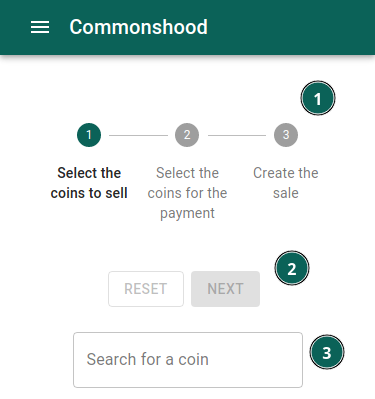
\includegraphics[width=\textwidth]{commonComponents.png}
          \caption{Componenti comuni}
          \centering
          \label{fig:commonComponents}
        \end{figure}
        Per mostrare graficamente il progresso nei diversi step è presente, in cima alla pagina, un componente
        \verb|<stepper>|, questo, come mostrato nell'immagine \ref{fig:commonComponents} al punto 1, indica all'utente gli step terminati e quelli ancora da completare.
        \newline
        Al di sotto, al punto 2, sono presenti due pulsanti per la navigazione nei vari step. Il primo permette di tornare allo step 1 azzerando tutti i parametri inseriti.
        Il secondo serve per avanzare allo step successivo.
        \newline
        Al punto 3 è presente un campo di inserimento per cercare una moneta in particolare. Questo componente è presente solo nel primo e secondo step
        \subsubsection{Caricamento della pagina}
        Al caricamento della pagina vengono inizializzate alcune variabili, tra cui le più significative sono le seguenti:
        \begin{lstlisting}[style=ES6, title={Inizializzazione delle variabili al caricamento della pagina Create Sale}]
        const {web3Instance, userAccount} = props;
        const [coinsToSellAmounts,
               setCoinsToSellAmounts] = useState(new Map());
        const [coinsToAcceptAmounts,
               setCoinsToAcceptAmounts] = useState(new Map());
        const [coinsList, setCoinsList] = useState([]);
        const [activeCoinsList,
               setActiveCoinsList] = useState([]);
        const [activeStep, setActiveStep] = useState(0);\end{lstlisting}
        \verb|web3Instance| contiene l'istanza di web3 mentre \verb|userAccount| contiene l'indirizzo Ethereum dell'utente corrente, questi vengono passati alla pagina come props.
        \newline
        \verb|coinsToSellAmounts| e \verb|coinsToAcceptAmounts| sono variabili dotate di stato ed entrambi sono di tipo \verb|Map|, ossia un dizionario con chiavi di ricerca e valori associati.
        Vengono usate per mantenere le quantità delle monete scelte da mettere in vendita, per la prima variabile, oppure quelle da accettare come pagamento, nel caso della seconda variabile.
        Hanno come chiavi di ricerca le monete mentre i valori sono le quantità di queste.
        \newline
        \verb|coinList| è un array usato per contenere la lista di tutte le monete possedute dall'account utente.
        \newline
        \verb|activeCoinsList| è l'array preso come riferimento per mostrare graficamente la lista delle monete.
        \newline
        \verb|activeStep| è un numero intero che indica lo step corrente.
        \newline
        Le variabili di stato hanno, naturalmente, associate le funzioni per modificarne il loro valore.
        \newline
        Una volta caricata la pagina, con l'uso di \verb|useEffect()|, viene richiamata la funzione \verb|fetchCoins|.
        \begin{lstlisting}[style=ES6, title={Funzione fetchCoins}]
        const fetchCoins = async () => {
          setLoadingCoinList(true)
          const newCoinsList = await coinGetListOnlyOwned(
                               web3Instance,userAccount);
          setLoadingCoinList(false);
          setCoinsList(newCoinsList);
          setActiveCoinsList(newCoinsList);
        }\end{lstlisting}

        \subsubsection{Box di ricerca}
        \begin{lstlisting}[style=ES6, title={Funzione fetchCoins}]
        const handleSearch = (event) => {
          const searchInput = event.target.value.toLowerCase();
  
          setActiveCoinsList(coinsList.filter(coin => {
              const coinName = coin.name.toLowerCase();
              const coinSymbol = coin.symbol.toLowerCase();
              if(coinName.includes(searchInput) || 
                 coinSymbol.includes(searchInput)) return coin;
          }));
        }

        <TextField 
        id="searchBox"
        label="Search for a coin"
        variant="outlined"
        onChange={handleSearch}/> \end{lstlisting}
        Il box di ricerca è realizzato usando il componente \verb|<TextField>|, ad ogni inserimento/eliminazione di caratteri viene invocata la funzione \verb|handleSearch|.
        Questa funzione, come visibile alla riga 1, prende come parametro l'evento lanciato. Quest'ultimo contiene il testo presente nel \verb|<TextField>|,
        questo viene, quindi, convertito in caratteri minuscoli ed assegnato alla variabile \verb|searchInput|. Alla riga 4 viene chiamata la funzione filter sull'array \verb|coinsList|,
        questo metodo ritorna un nuovo array dopo aver filtrato gli elementi della lista secondo un certo criterio. In questo caso, il criterio, visibile alle righe 7 e 8,
        è che il nome o il simbolo della moneta che si sta controllando contenga la stringa da cercare contenuta in \verb|searchInput|. In caso positivo la moneta viene aggiunta all'array da ritornare.
        Una volta terminata la funzione di filtro si ha quindi una lista contenete solo monete che includono il termine di ricerca. Dopodichè questa lista viene assegnata alla variabile di stato \verb|activeCoinsList| usando,
        perciò, la funzione \verb|setActiveCoinsList()|. In questo modo verranno mostrate a video le monete filtrate. 

        \subsubsection{Step 1: scelta dei token da vendere}
        \begin{figure}[H]
          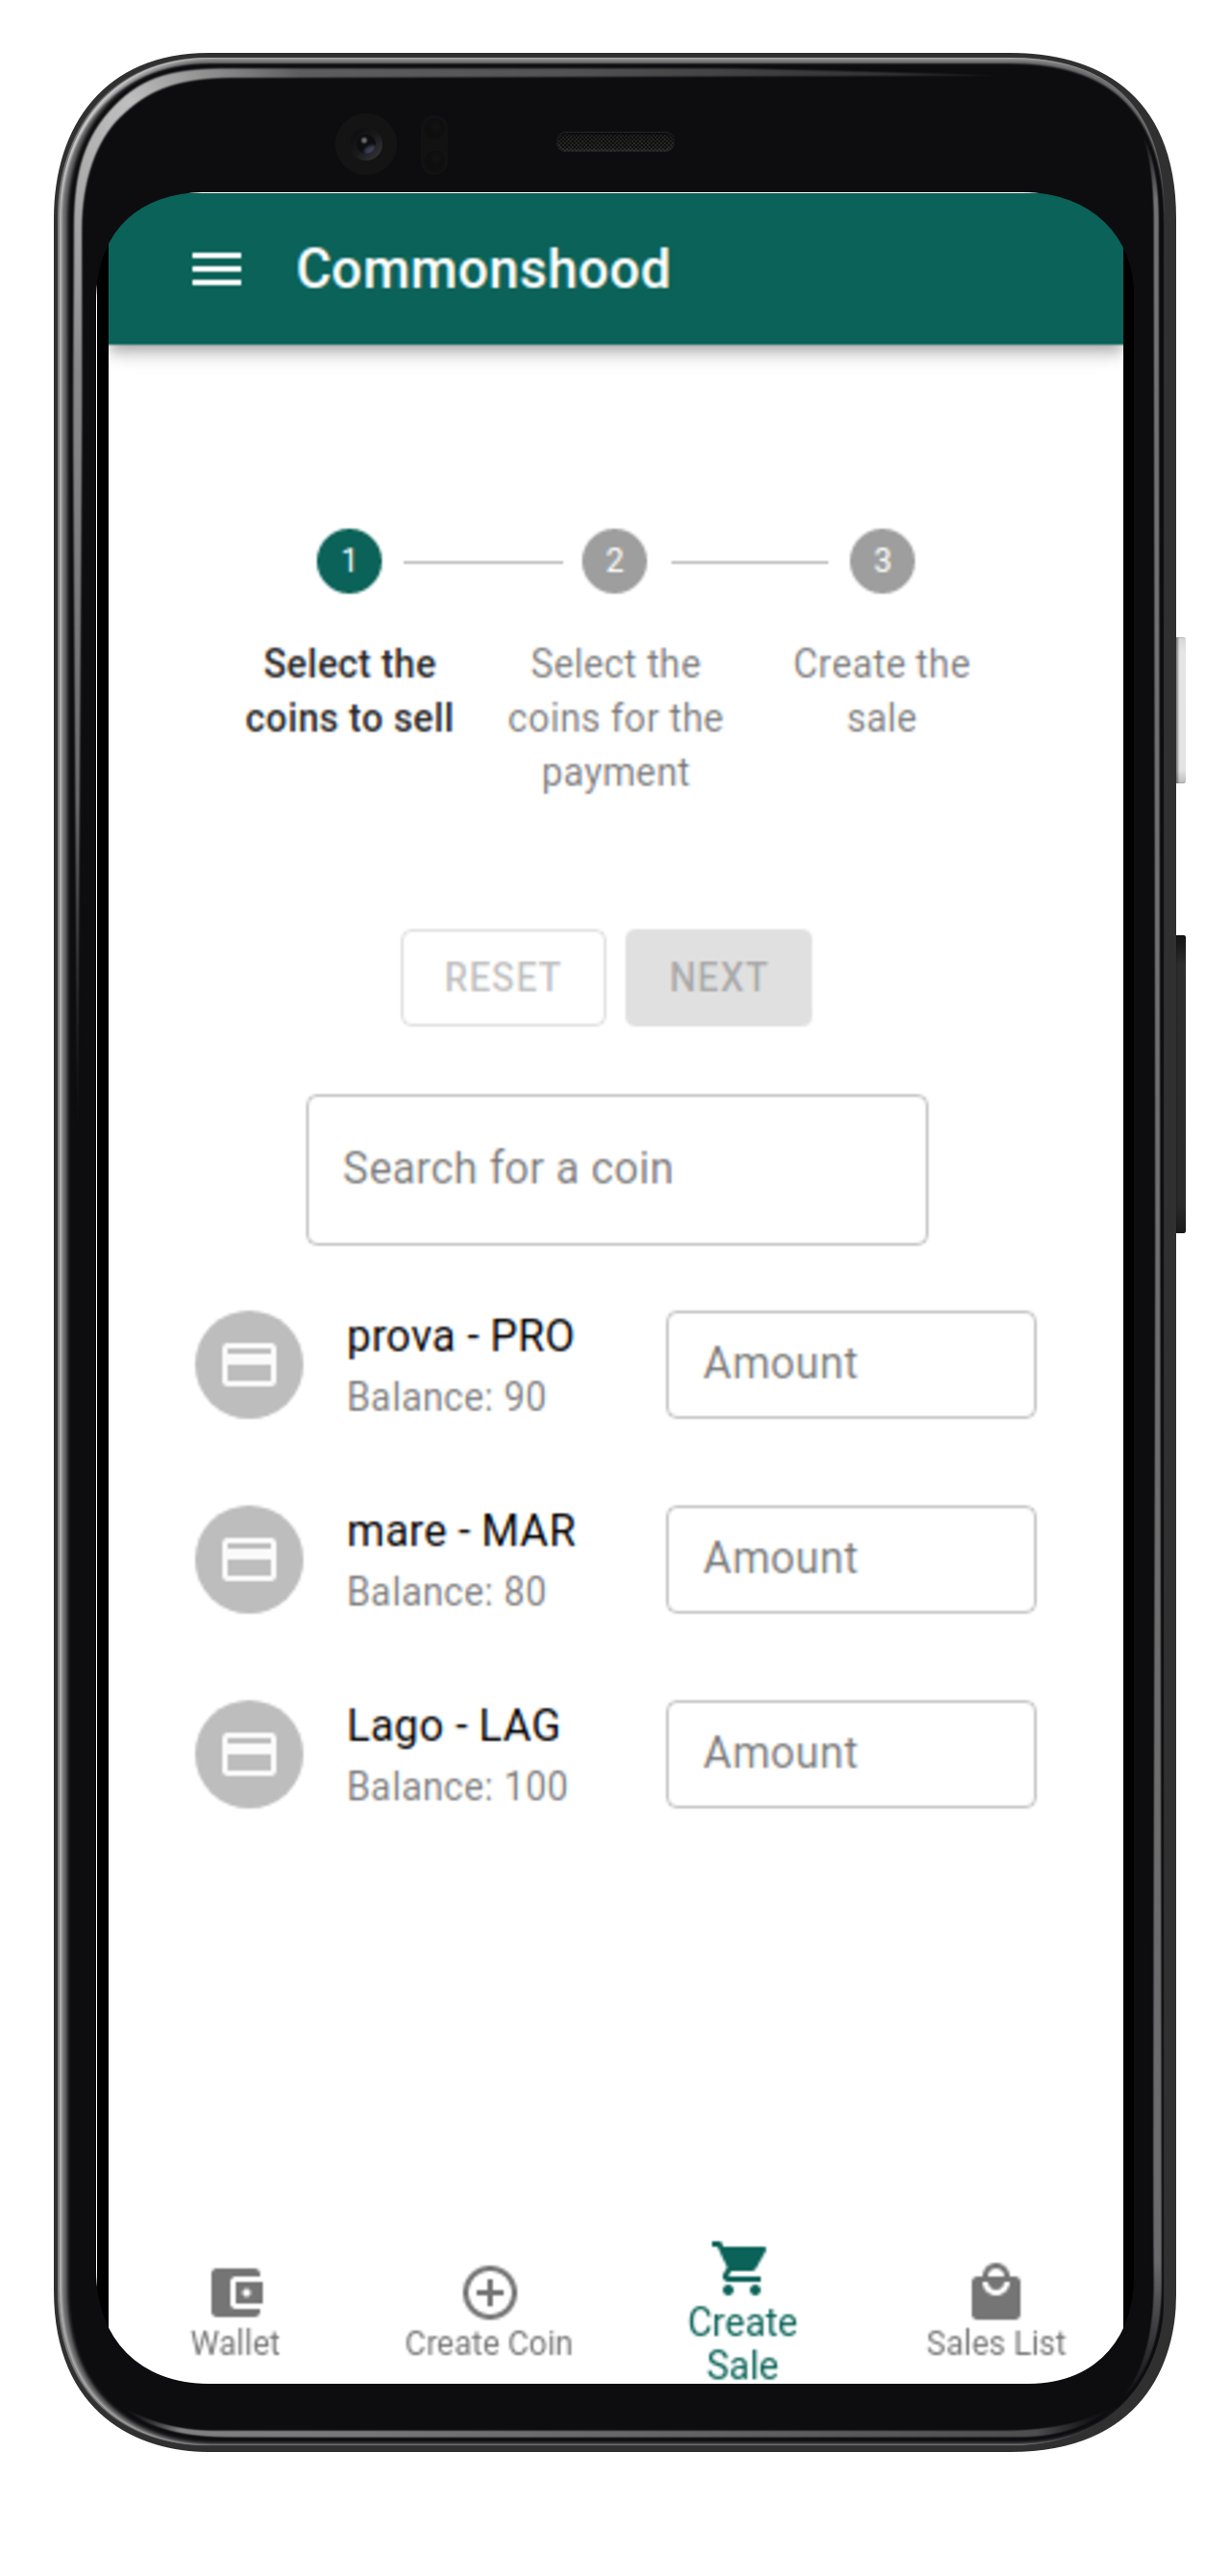
\includegraphics[width=\textwidth]{coinsToSell.png}
          \caption{Pagina per la scelta dei token in vendita}
          \centering
          \label{fig:selectCoinsToSell}
        \end{figure}
        La pagina, visibile in figura \ref{fig:selectCoinsToSell}, contiene un componente custom chiamato \verb|SelectCoins|, questo ha come props l'array \verb|activeCoinsList| e genera, usando il componente \verb|<List>|, una lista contenente tutte le monete della lista.
        \newline
        Ogni elemento della lista contiene le informazioni di un token all'interno di \verb|activeCoinsList| e un componente
        \verb|<TokenListItem>| contenente un componente \verb|<TextField>|. Quest'ultimo permette l'inserimento della quantità desiderata del token da mettere in vendita.
        \paragraph{Inserimento di una quantità di una moneta}
        \label{insertCoinsToSell}
        \begin{lstlisting}[style=ES6, title={Funzione handleAmountChange}]
const handleAmountChange = (coin, amount) => {
  const isInputEmpty = amount.length === 0;
  amount = parseInt(amount);

  if(isInputEmpty || amount === 0) {
    const newMap = new Map(coinsToSellAmounts);
    newMap.delete(coin);
    setCoinsToSellAmounts(newMap);
  } else {
    setCoinsToSellAmounts(prev => new Map(prev.set(coin, amount)));
  }

  if(amount > coin.balance) {
    setErrorsAmounts(prev => new Set(prev.add(coin)));
  } else {
    const newSet = new Set(errorsAmounts);
    newSet.delete(coin);
    setErrorsAmounts(newSet);
  }
}\end{lstlisting}
        All'inserimento della quantità di una moneta viene richiamata la funzione \verb|handleAmountChange(coin, amount)| passando, come paramentri, la moneta interessata e la quantità inserita.
        \newline
        La funzione inizia assegnando alla variabile \verb|isInputEmpty| il valore \verb|true| in caso il parametro \verb|amount| sia una stringa vuota, \verb|false| altrimenti. Inoltre, siccome \verb|amount| è una stringa, converte questo in un valore intero.
        \newline
        Successivamente, in caso \verb|isInputEmpty| sia \verb|true| oppure \verb|amount| sia 0, viene eliminato da \verb|coinsToSellAmounts| la voce con chiave di ricerca \verb|coin|. Altrimenti inserisce, sempre in \verb|coinsToSellAmounts|, una voce con chiave \verb|coin| e valore \verb|amount|.
        In questo modo \verb|coinsToSellAmounts| contiene sempre le monete e le quantità associate inserite dall'utente.
        \newline
        La funzione, inoltre, controlla che la quantità inserita non ecceda la quantità posseduta dall'utente, ossia confronta \verb|amount| e il parametro \verb|balance| all'interno di \verb|coin|.
        \newline
        Nel caso di \verb|amount| maggiore di \verb|coin.balance|, cioè l'utente non possiede la quantità inserita, viene aggiunto a \verb|errorsAmounts| il valore l'oggetto \verb|coin|.
        Nel caso opposto viene eliminato \verb|coin| da \verb|errorsAmounts|. \verb|errorsAmounts| viene poi utilizzato, in caso di errore nell'inserimento di una quantità, per disabilitare il bottone per passare al prossimo step.
        Per far questo basta controllare che \verb|errorsAmounts| non sia vuoto.
        \paragraph{Quantità errata}
        \label{quantityerror}
        \begin{figure}[ht]
          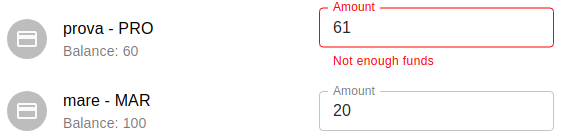
\includegraphics[scale=0.5]{errorMessage.png}
          \centering
          \caption{Sopra un inserimento di quantità errata, sotto un inserimento corretto}
          \label{fig:errorMessage}
        \end{figure}
        Il componente \verb|SelectCoins| ha una props chiamata \verb|showCoinError| a cui viene passato il riferimento ad una funzione chiamata \verb|showCoinError()|.
        \begin{lstlisting}[style=ES6, title={Funzione showCoinError}]
const showCoinError = (coin, balance) => {
  if(activeStep === 0) 
    if(coinsToSellAmounts.has(coin) && coinsToSellAmounts.get(coin) > balance)
      return true;
  return false;
}\end{lstlisting}
        Questa funzione prende in input due parametri: \verb|coin|, ossia una moneta, e \verb|balance|, la quantità di \verb|coin| che l'utente possiede. La funzione inizia controllando che l'attuale step sia lo 0,
        questo perché è solo nello step iniziale che possono presentarsi errori nell'inserimento di quantità. La funzione prosegue, quindi, controllando che \verb|coinsToSellAmounts| abbia l'oggetto \verb|coin|, e che il valore associato a \verb|coin| in \verb|coinsToSellAmounts| sia superiore a \verb|balance|.
        In questo caso vuol dire che l'utente ha inserito \verb|coin| tra le monete da vendere, ma ha inserito una quantita che non possiede, quindi la funzione restituisce \verb|true|.
        \newline
        Il componente \verb|<SelectCoins>| quando genera i vari \verb|<TokenListItem>| di ogni moneta, ossia i componenti che contengono i box di inserimento delle quantità, aggiunge loro una props \verb|showError| contenente la chiamata alla funzione \verb|showCoinError()|,
        passando la moneta e il bilancio della moneta.
        \begin{lstlisting}[style=ES6, title={Funzione showCoinError}]
  <TokenListItem 
  showError={props.showCoinError(coin, coin.balance)}
  ... 
  />
\end{lstlisting}
        Dove \verb|coin| è ottenuto facendo ciclo sull'array \verb|activeCoinsList|.
        \newline
        Ogni \verb|<TokenListItem>| ha un valore di tipo boolean all'interno della proprietà \verb|showError|. Questo viene usato per scegliere se mostrare la \verb|<TextField>| di inserimento con messaggio di errore oppure normale, come visibile in figura \ref{fig:errorMessage}.
\begin{lstlisting}[style=ES6, title={Scelta di TextField da mostrare}]
(props.showError) ?
<TextField error={true} helperText={errorMessage} .../>
:
<TextField .../>\end{lstlisting}
        \paragraph{Avanzamento al passo 2}
        Cliccando sul pulsante \verb|next|, oltre a passare al passo successivo, vengono effettuate le seguenti operazioni.
\begin{lstlisting}[style=ES6, title={Codice eseguito passando al passo 2}]
let newCoinsList = await coinGetListAll(web3Instance, userAccount);
const selectedCoins = Array.from(coinsToSellAmounts.keys());
newCoinsList = newCoinsList.filter(coin => {
    for(let c of selectedCoins) {
        if(c.address === coin.address) return false;
    }
    return true;
});
setLoadingCoinList(false);
setCoinsList(newCoinsList);
setActiveCoinsList(newCoinsList);\end{lstlisting}
        Questo codice genera un array \verb|newCoinsList| contenente tutte le monete tranne quelle che l'utente ha selezionato di vendere al passo 1. Questo array viene, quindi, assegnato a \verb|coinsList| e \verb|activeCoinsList|.

        \subsubsection{Step 2: scelta dei token da accettare}
        Il processo di scelta dei token da accettare come pagamento è molto simile a quello della scelta dei token da vendere del primo step. La principale differenza è l'array \verb|activeCoinsList| passato a \verb|SelectCoins|.
        Questo, infatti, nel passo 2 non contiene solo le monete possedute dall'utente, ma contiene tutte le monete tranne quelle che l'utente ha selezionato nello step 1.
        \newline
        Inoltre non è più necessario controllare la quantità inserita perché non c'è la restrizione del bilancio dell'utente, perciò il sistema descritto in \ref{quantityerror} non è applicato in questo step.
        Naturalmente la funzione \verb|handleAmountChange()|, richiamata ad ogni inserimento/modifica di una quantità, non modifica più \verb|coinsToSellAmounts|, come in \ref{insertCoinsToSell}, ma modifica \verb|coinsToAcceptAmounts|.

        \subsubsection{Step 3: sommario finale}

        \newpage
        \printbibliography
\end{document}